\documentclass{tudelft-report}

%% Set up the bibliography
\usepackage{biblatex}
\addbibresource{report.bib}

%% Additional packages and commands
\usepackage{parskip}
\setlist{itemsep=-2pt} % Reducing white space in lists slightly
\renewcommand{\deg}{\si{\degree}\xspace} % Use \deg easily, everywhere
\usepackage{tcolorbox}

%% ----------------------------------------------------------------------
%%    Begin of document + Frontmatter (Roman page numbering)
%% ----------------------------------------------------------------------

\begin{document}

\frontmatter

%% Define the main parameters
\title{\textbf{Laboratorio} \\ Detección de Movimiento y Seguimiento de Objetos}
\author{Ingeniería Matemática}

\subject{Visión por Ordenador I} % Cover only
\affiliation{Universidad Pontificia Comillas, ICAI} % Cover only
\coverimage{figures/cover.jpg} % Aspect ratio of 2:3 (portrait) recommended
\definecolor{title}{HTML}{ffffff} % Color for cover title

\makecover

\begin{titlepage}

\begin{center}

\bigskip
\bigskip

%% Print the name of the author
{\makeatletter
\begin{tabular}{c}
    3º \@author \\\midrule
    Curso 2024/25
\end{tabular}
\makeatother}

\bigskip
\bigskip

%% Print the title
{\makeatletter
\largetitlestyle\fontsize{45}{45}\selectfont\@title
\makeatother}

%% Print the subtitle
{\makeatletter
\ifdefvoid{\@subtitle}{}{\bigskip\titlestyle\fontsize{20}{20}\selectfont\@subtitle}
\makeatother}

%% Print table with names; easily add columns if necessary or remove the table completely
% \setlength\extrarowheight{2pt}
% \begin{tabular}{c}
%     3º  \\\midrule
%     Curso 2024/25 \\
% \end{tabular}

\vfill

%% Print some more information at the bottom
\begin{tabular}{ll}
    \textbf{Profesor}: & \textbf{Email} \\
    Erik Velasco & evelasco@icai.comillas.edu \\
    Lionel Güitta & lglopez@icai.comillas.edu \\
    Daniel Pinilla & dpinilla@icai.comillas.edu \\
    Luis Arias & learias@icai.comillas.edu \\
    Rodrigo Sánchez & rsmolina@icai.comillas.edu \\ 
    Ignacio de Rodrigo & iderodrigo@comillas.edu \\
\end{tabular}

\bigskip
\bigskip

%% Add a source and description for the cover and optional attribution for the template
\begin{tabular}{p{15mm}p{10cm}}
    Cover: &Tiny satellites, also known as CubeSats, are pictured after being deployed into Earth orbit from a small satellite orbital deployer on the outside of the International Space Station's Kibo laboratory module. Image Credit: NASA/Tracy Dyson \\
    % Feel free to remove the following attribution, it is not required - still appreciated :-)
    % Style: & TU Delft Report Style, with modifications by Daan Zwaneveld
\end{tabular}
\vspace{10mm}

\end{center}

%% Insert the Comillas logo at the bottom of the page
\begin{tikzpicture}[remember picture, overlay]
    \node[above=10mm] at (current page.south) {%
        
\includegraphics[scale=0.15]{figures/logo-color}
    };
\end{tikzpicture}

\end{titlepage}

%\input{frontmatter/preface}
%\input{frontmatter/summary}

\tableofcontents
%\listoffigures
%\listoftables

%\input{frontmatter/nomenclature}

%% ----------------------------------------------------------------------
%%    Mainmatter (Arabic page numbering)
%% ----------------------------------------------------------------------

\mainmatter

\chapter{Sesión 4: Detección de Movimiento y Seguimiento de Objetos}
\label{chapter:introduction_ses_4}

\section{Materiales}

En esta práctica se trabajará con los siguientes recursos (puede encontrarlos en la sección de Moodle \textit{Laboratorio/Sesión 4}):

\begin{itemize}
    \item \textbf{\texttt{lab4.ipynb}}: notebook con el código que deberá desarrollar.
    \item \textbf{data}: carpeta con vídeos para trabajar durante la práctica.
\end{itemize}

\section{Apartados de la práctica}

La Sesión 4 del laboratorio está dividida en los siguientes apartados:

\begin{itemize}
    \item Librerías: Importación de las librerías que se utilizan en la sesión. Se recomienda realizar la importación en una celda inicial para mantener la organización del Notebook.
    \item Apartado A: Sustracción de fondo.
    \item Apartado B: Flujo Óptico.
    \item Apartado D: Filtro de Kalman para Seguimiento de Objetos.
    \item Apartado D: Ejercicio Adicional.
\end{itemize}

\section{Observaciones}

Aunque el guion de la práctica y los comentarios en Markdown del Notebook estén escritos en español, observe que todo aquello que aparece en las celdas de código está escrito en inglés. Es una buena práctica que todo su código esté escrito en inglés.

Aquellas partes del código que deberá completar están marcadas con la etiqueta \textbf{\texttt{TODO}}.

Es muy importante que trabaje consultando la documentación de OpenCV\footnote{\href{https://docs.opencv.org/4.x/index.html}{Documentación de OpenCV}: \url{https://docs.opencv.org/4.x/index.html}} para familiarizarse de cara al examen. Tenga en cuenta que en los exámenes no podrá utilizar herramientas de ayuda como Copilot.

\section{Qué va a aprender}

Al finalizar esta práctica, aprenderá a implementar algoritmos de detección de movimiento mediante sustracción de fondo y flujo óptico, y explorará el filtro de Kalman para el seguimiento de objetos.

\section{Evaluación}

La nota que obtenga en esta sesión de laboratorio será la misma que obtenga su pareja. Los apartados de la práctica serán evaluados como refleja la Tabla \ref{table:evaluacion}.

\begin{table}[h!]
    \centering
    \begin{tabular}{|c|c|c|}
    \hline
    \textbf{Tarea} & \textbf{Valor} & \textbf{Resultado} \\
    \hline
    Pregunta A.1 & 1.5 & \\
    \hline
    Pregunta A.2 & 2.0 & \\
    \hline
    Pregunta B.1 & 1.5 & \\
    \hline
    Pregunta B.2 & 2.0 & \\
    \hline
    Pregunta C.1 & 1.5 & \\
    \hline
    Pregunta C.2 & 1.5 & \\
    \hline
    Pregunta D.1 & 1.0 & \\
    \hline
    Pregunta D.2 & 1.0 & \\
    \hline
    \textbf{Total} & \textbf{12.0} & \\
    \hline
    \end{tabular}
    \caption{Valoración de los apartados de la práctica.}
    \label{table:evaluacion}
\end{table}

\chapter{Apartado A: \textbf{Sustracción de Fondo}}
\label{chapter:tarea_a}


\section*{Tarea A.1: Carga de vídeo}
\phantomsection
\addcontentsline{toc}{section}{Tarea A.1: Carga de vídeo}
Cargue el vídeo (\texttt{'visiontraffic.avi'}) en el cual se detectarán objetos en movimiento. Para ello, realice complete el método \texttt{read\_video} que puedrá reutilizar en el resto de tareas. 

\section*{Tarea A.2: Sustracción de fondo mediante diferencia de frames}
\phantomsection
\addcontentsline{toc}{section}{Tarea A.2: Sustracción de fondo mediante diferencia de frames}
Realice una sustracción de fondo mediante diferencia de frames, para ello guarde un frame con el fondo estático y úselo como frame de referencia de fondo.

En primer lugar vamos a iterar sobre la lista de frames para mostrar por pantalla frame a frame e iremos avanzando con pulsando la tecla n, para seleccionar el frame de referencia debera pulsar la tecla s.

Posteriormente se realizará la diferencia de frames entre el frame referencia y el frame actual.

\begin{figure}[H]
    \centering
    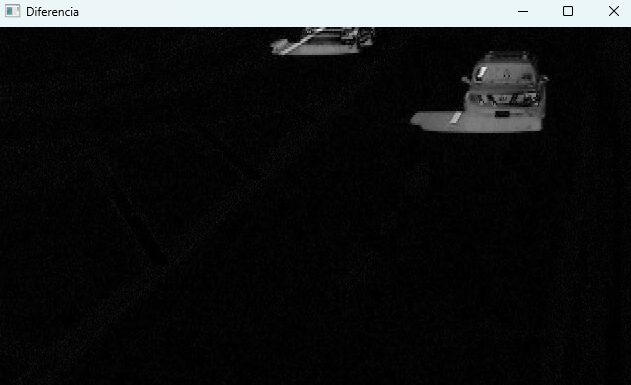
\includegraphics[width=0.3\textwidth]{Lab_4/template/figures/frame_difference.png}
    \caption{Ejemplo de resultado con diferencia de frames.}
    \label{fig:ejemplo_framediff}
\end{figure}

\section*{Tarea A.3: Configuración de la Sustracción de Fondo con GMM}
\phantomsection
\addcontentsline{toc}{section}{Tarea A.3: Configuración de la Sustracción de Fondo con GMM}

Configure el sustractor de fondo usando el modelo de mezcla de gaussianas adaptativas (MOG2). Para ello, usaremos \texttt{cv2.createBackgroundSubtractorMOG2}\footnote{ \href{https://docs.opencv.org/4.8.0/d7/d7b/classcv_1_1BackgroundSubtractorMOG2.html}{Documentación del método MOG2 en OpenCV:} \\{https://docs.opencv.org/4.8.0/d7/d7b/classcv\_1\_1BackgroundSubtractorMOG2.html}}

\section*{Tarea A.4: Aplicación de la Sustracción de Fondo}
\phantomsection
\addcontentsline{toc}{section}{Tarea A.4: Aplicación de la Sustracción de Fondo}
Aplique la sustracción de fondo en cada frame para extraer los objetos en movimiento.


Visualice el resultado de la detección de movimiento y guarde el vídeo con las imagenes binarias resultantes en la carpeta \texttt{data/results}. Utilize el método \texttt{cv2.VideoWriter}\footnote{ \href{https://docs.opencv.org/4.8.0/dd/d9e/classcv_1_1VideoWriter.html}{Documentación del método MOG2 en OpenCV:} \\{https://docs.opencv.org/4.8.0/dd/d9e/classcv\_1\_1VideoWriter.html}}

\begin{figure}[H]
    \centering
    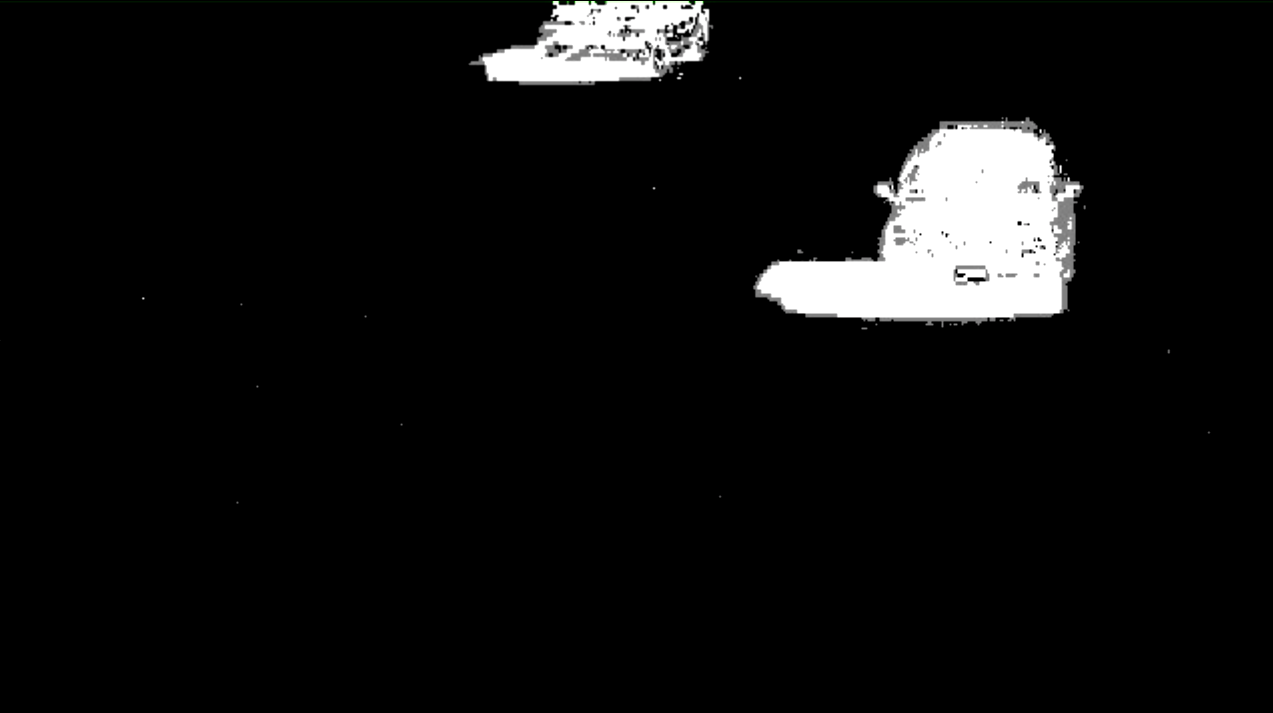
\includegraphics[width=0.3\textwidth]{Lab_4/template/figures/MOG2.png}
    \caption{Ejemplo de resultado usando MOG2.}
    \label{fig:ejemplo_mog2}
\end{figure}

\section*{Preguntas}
\addcontentsline{toc}{section}{Preguntas}

\vspace{5mm}
\begin{tcolorbox}[colback=gray!10, colframe=gray!30, coltitle=black, title=Pregunta A.1, halign=left]
¿Cómo afecta la variable \texttt{varThreshold} a la precisión de la detección?
\end{tcolorbox}

\vspace{5mm}
\begin{tcolorbox}[colback=gray!10, colframe=gray!30, coltitle=black, title=Pregunta A.2, halign=left]
¿Qué ventajas presenta \texttt{createBackgroundSubtractorMOG2} frente a métodos simples de diferencia de imágenes?
\end{tcolorbox}
\chapter{Apartado B: \textbf{Flujo Óptico}}
\label{chapter:tarea_b}

\section*{Tarea B.1: Configuración del Flujo Óptico}
\phantomsection
\addcontentsline{toc}{section}{Tarea B.1: Configuración del Flujo Óptico}
Para esta tarea vamos a utilizar el video (\texttt{'slow\_traffic\_small.mp4'}), para cargarlo utilice el método que se ha desarrollado anteriormente.
Implemente el flujo óptico de Lucas-Kanade, útil para detectar el movimiento pixel a pixel. Para ello vamos a comenzar por definir los parametros necesarios para utilizar el método \texttt{cv2.calcOpticalFlowPyrLK}\footnote{ \href{https://docs.opencv.org/4.8.0/dc/d6b/group\_\_video\_\_track.html\#ga473e4b886d0bcc6b65831eb88ed93323}{Documentación del método Optical Flow Lucas-Kanade en OpenCV:} \\{https://docs.opencv.org/4.8.0/dc/d6b/group\_\_video\_\_track.html\#ga473e4b886d0bcc6b65831eb88ed93323}}

\section*{Tarea B.2: Detección de Puntos de Interés}
\phantomsection
\addcontentsline{toc}{section}{Tarea B.2: Detección de Puntos de Interés}
Configure los párametros para obtener los puntos de interés iniciales en el primer frame con el método de \texttt{cv2.goodFeaturesToTrack}\footnote{ \href{https://docs.opencv.org/4.8.0/dd/d1a/group\_\_imgproc\_\_feature.html\#ga1d6bb77486c8f92d79c8793ad995d541}{Documentación del método Optical Flow Lucas-Kanade en OpenCV:} \\{https://docs.opencv.org/4.8.0/dd/d1a/group\_\_imgproc\_\_feature.html\#ga1d6bb77486c8f92d79c8793ad995d541}}.

\section*{Tarea B.3: Cálculo y Visualización del Flujo Óptico}
\phantomsection
\addcontentsline{toc}{section}{Tarea B.3: Cálculo y Visualización del Flujo Óptico}
Calcule el flujo óptico con el método de Lucas-Kanade aplicando \texttt{cv2.calcOpticalFlowPyrLK} y visualice el movimiento de cada punto de interés en los siguientes frames.

\begin{figure}[H]
    \centering
    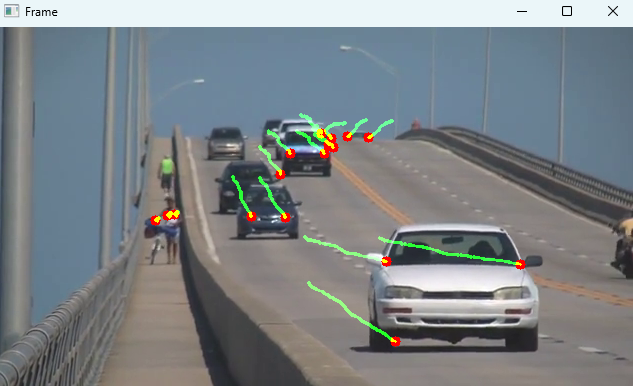
\includegraphics[width=0.3\textwidth]{Lab_4/template/figures/of_lk.png}
    \caption{Ejemplo de resultado de obtener el flujo ópitco con el metodo de Lucas-Kanade.}
    \label{fig:ejemplo_opticalflowLK}
\end{figure}

\section*{Preguntas}
\addcontentsline{toc}{section}{Preguntas}

\vspace{5mm}
\begin{tcolorbox}[colback=gray!10, colframe=gray!30, coltitle=black, title=Pregunta B.1, halign=left]
¿Qué efecto tiene el parámetro \texttt{winSize} en la precisión del flujo óptico?
\end{tcolorbox}


\vspace{5mm}
\begin{tcolorbox}[colback=gray!10, colframe=gray!30, coltitle=black, title=Pregunta B.2, halign=left]
¿Cómo influye el parámetro \texttt{qualityLevel} en la función \texttt{cv2.goodFeaturesToTrack} al detectar puntos de interés?
\end{tcolorbox}
\chapter{Apartado C: \textbf{Filtro de Kalman para Seguimiento de Objetos}}
\label{chapter:tarea_c}

\section*{Tarea C.1: Configuración del Filtro de Kalman}
\phantomsection
\addcontentsline{toc}{section}{Tarea C.1: Configuración del Filtro de Kalman}
Para esta tarea vamos a utilizar el video (\texttt{'slow\_traffic\_small.mp4'}), para cargarlo utilice el método que se ha desarrollado anteriormente. Inicialice el filtro de Kalman, para ello haga uso del método \texttt{cv2.KalmanFilter}\footnote{ \href{https://docs.opencv.org/4.8.0/dd/d6a/classcv_1_1KalmanFilter.html}{Documentación del método KalmalFilter en OpenCV:} \\{https://docs.opencv.org/4.8.0/dd/d6a/classcv\_1\_1KalmanFilter.html}} de Opencv, con una matriz de medición y transición adecuada para un seguimiento en dos dimensiones.

Complete el código del bucle que nos permitirá seleccionar el objeto \texttt{(cv2.selectROI)}\footnote{ \href{https://docs.opencv.org/4.8.0/d7/dfc/group\_\_highgui.html\#gaabb58bae304674b429d9102a7155a86e}{Documentación del método para seleccionar la ROI en OpenCV:} \\{https://docs.opencv.org/4.8.0/d7/dfc/group\_\_highgui.html\#gaabb58bae304674b429d9102a7155a86e}} que vamos a seguir. Convierta la región de interés de la imagen a HSV y calcule el histograma \texttt{cv2.calcHist}\footnote{ \href{https://docs.opencv.org/4.8.0/d6/dc7/group\_\_imgproc\_\_hist.html\#ga4b2b5fd75503ff9e6844cc4dcdaed35d}{Documentación del método para calculo de histograma en OpenCV:} \\{https://docs.opencv.org/4.8.0/d6/dc7/group\_\_imgproc\_\_hist.html\#ga4b2b5fd75503ff9e6844cc4dcdaed35d}} con  para el canal con la información de tono (\textit{Hue}).

\begin{figure}[H]
    \centering
    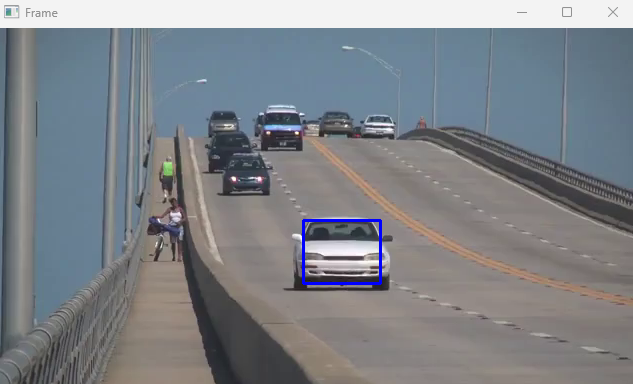
\includegraphics[width=0.3\textwidth]{Lab_4/template/figures/roi_selection.png}
    \caption{Ejemplo de ROI.}
    \label{fig:ejemplo_ROI_kalman}
\end{figure}

\section*{Tarea C.2: Predicción y Corrección del Estado}
\phantomsection
\addcontentsline{toc}{section}{Tarea C.2: Predicción y Corrección del Estado}
Realice la predicción del estado y corrija la posición estimada en cada iteración.

\begin{figure}[H]
    \centering
    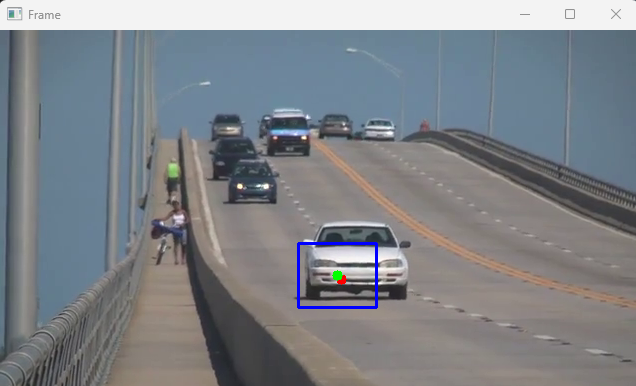
\includegraphics[width=0.3\textwidth]{Lab_4/template/figures/kalman.png}
    \caption{Ejemplo de seguimiento con filtro de Kalman.}
    \label{fig:ejemplo_track_kalman}
\end{figure}

\section*{Preguntas}
\addcontentsline{toc}{section}{Preguntas}

\vspace{5mm}
\begin{tcolorbox}[colback=gray!10, colframe=gray!30, coltitle=black, title=Pregunta C.1, halign=left]
¿Cómo afecta el valor de \texttt{transitionMatrix} a la predicción en el filtro de Kalman?
\end{tcolorbox}

\vspace{5mm}
\begin{tcolorbox}[colback=gray!10, colframe=gray!30, coltitle=black, title=Pregunta C.2, halign=left]
¿Cuál es la diferencia entre \texttt{measurementMatrix} y \texttt{transitionMatrix} en el contexto del seguimiento de objetos?
\end{tcolorbox}
\chapter{Ejercicio Adicional: \textbf{Exploración del Modelo de Mezcla de Gaussianas (GMM)}}
\label{chapter:tarea_d}

Esta sección es completamente voluntaria y puede realizarla para mejorar su puntuación en la práctica.

\subsection*{Objetivo}
Investigue cómo funciona el modelo de mezcla de gaussianas (GMM) para mejorar la detección en condiciones de iluminación cambiantes.

\begin{enumerate}
    \item \textbf{Implementación del GMM}: Utilice \texttt{cv2.createBackgroundSubtractorMOG()} y ajuste el parámetro \texttt{history} para observar cómo cambia la detección en función de la duración de la memoria del fondo.
    \item \textbf{Comparación con MOG2}: Observe las diferencias en la sensibilidad a las sombras y los cambios de iluminación. Pruebe con vídeos que incluyan cambios graduales de iluminación y objetos que se detienen temporalmente.
\end{enumerate}

\section*{Preguntas}
\addcontentsline{toc}{section}{Preguntas}

\vspace{5mm}
\begin{tcolorbox}[colback=gray!10, colframe=gray!30, coltitle=black, title=Pregunta D.1, halign=left]
¿Qué ventajas observa en \texttt{createBackgroundSubtractorMOG} en comparación con \texttt{createBackgroundSubtractorMOG2}?
\end{tcolorbox}

\vspace{5mm}
\begin{tcolorbox}[colback=gray!10, colframe=gray!30, coltitle=black, title=Pregunta D.2, halign=left]
¿Cómo afecta el parámetro \texttt{history} al rendimiento de detección en escenas con objetos que aparecen y desaparecen?

\vspace{3mm}
Al finalizar este ejercicio, agregue las observaciones y las imágenes generadas en el informe final de la práctica para una evaluación completa de los resultados.
\end{tcolorbox}


%% Prevent urls running into margins in bibliography
\setcounter{biburlnumpenalty}{7000}
\setcounter{biburllcpenalty}{7000}
\setcounter{biburlucpenalty}{7000}

%% Add bibliography
% \printbibliography[heading=bibintoc,title=References]

%% ----------------------------------------------------------------------
%%    Appendix (Letters for chapters)
%% ----------------------------------------------------------------------

%\appendix

%\chapter{Source Code Example}
%\label{chapter:title}

\emph{Adding source code to your report/thesis is supported with the package {\normalfont\texttt{listings}}. An example can be found below. Files can be added using {\normalfont\texttt{\textbackslash lstinputlisting[language=<language>]\{<filename>\}}}.}

\begin{lstlisting}[language=Python]
"""
ISA Calculator: import the function, specify the height and it will return a
list in the following format: [Temperature,Density,Pressure,Speed of Sound].
Note that there is no check to see if the maximum altitude is reached.
"""

import math
g0 = 9.80665
R = 287.0
layer1 = [0, 288.15, 101325.0]
alt = [0,11000,20000,32000,47000,51000,71000,86000]
a = [-.0065,0,.0010,.0028,0,-.0028,-.0020]

def atmosphere(h):
    for i in range(0,len(alt)-1):
        if h >= alt[i]:
            layer0 = layer1[:]
            layer1[0] = min(h,alt[i+1])
            if a[i] != 0:
                layer1[1] = layer0[1] + a[i]*(layer1[0]-layer0[0])
                layer1[2] = layer0[2] * (layer1[1]/layer0[1])**(-g0/(a[i]*R))
            else:
                layer1[2] = layer0[2]*math.exp((-g0/(R*layer1[1]))*(layer1[0]-layer0[0]))
    return [layer1[1],layer1[2]/(R*layer1[1]),layer1[2],math.sqrt(1.4*R*layer1[1])]
\end{lstlisting}

%\chapter{Task Division Example}
%\label{chapter:title}

\emph{If a task division is required, a simple template can be found below for convenience. Feel free to use, adapt or completely remove.}

\begin{table}[htb]
    \setlength\extrarowheight{4pt}
    \centering
    \caption{Distribution of the workload}
    \label{tab:taskdivision}
    \begin{tabularx}{\textwidth}{lXX}
        \toprule
        & Task & Student Name(s) \\
        \midrule
        & Summary & \\
        Chapter 1 & Introduction &  \\
        Chapter 2 &  & \\
        Chapter 3 &  & \\
        Chapter * &  & \\
        Chapter * & Conclusion &  \\
        \midrule
        & Editors & \\
        & CAD and Figures & \\
        & Document Design and Layout & \\
        \bottomrule
    \end{tabularx}
\end{table}

%\input{appendix/appendix-c} % Create file to add

\end{document}
